\section{Results}
\label{sec:results}

In this section we demonstrate the capabilities of \textsc{PineAPPL} by
computing fast interpolation grids, accurate to NLO QCD and NLO QCD+EW,
for a representative set of processes in which EW corrections are expected 
to be sizeable. In order to consider some realistic kinematics for these
processes, we resort to measurements commonly devised for inclusion in PDF
fits. Our aim is twofold. On the one hand, we want to validate the results
obtained with \textsc{PineAPPL}; on the other hand, we want to assess the
impact of the EW corrections for usual experimental setups. We describe first
the processes and measurements that we consider, then the computational
settings that we adopt, and finally the results that we obtain.

\subsection{Processes and measurements}
\label{subsec:processes_and_measurements}

We focus on the following three processes: DY lepton-pair production, top-quark
pair production, and Z-boson (lepton-pair) production with non-zero transverse
momentum at the LHC. For each of these processes, we consider the measurements
described below.

\paragraph{DY lepton pair production.}
We select the distribution, single-differential in the invariant mass of the
lepton pair, $M_{\ell \bar\ell}$, measured by the ATLAS experiment at a centre-of
mass energy of 7~TeV in the high-mass region
($M_{\ell\bar\ell}>116$~GeV)~\cite{Aad:2013iua}.
We also select the distribution, double-differential in the rapidity and in
the invariant mass of the lepton pair, $y_{\ell\bar\ell}$ and $M_{\ell\bar\ell}$,
measured by the CMS experiment at a centre-of-mass energy of
7~TeV~\cite{Chatrchyan:2013tia}.
These measurements are currently included as standard in the
NNPDF3.1~\cite{Ball:2017nwa} and MMHT2014~\cite{Harland-Lang:2014zoa} PDF sets,
although with appropriate kinematic cuts that remove the bins at the largest
values of invariant mass, where EW corrections become sizeable.

\paragraph{Top-quark pair production.}
We select the distributions, single-differential in either the transverse
momentum of the top quark, $p_T^t$, or the invariant mass of the top-quark
pair, $m_{t\bar t}$, measured by the ATLAS and CMS experiments at a centre-of-mass
energy of 8~TeV~\cite{Aad:2015mbv,Khachatryan:2015oqa}. These measurements have
been extensively studied in the context of PDF fits in
Refs.~\cite{Czakon:2016olj,Bailey:2019yze,Amoroso:2020lgh,Kadir:2020yml}, and
included by default in the CT18~\cite{Hou:2019efy} analysis.
Because EW corrections are significantly smaller for distributions differential
in the rapidity of either the top quark or the top-quark
pair~\cite{Czakon:2017wor}, these distributions were preferred for inclusion
in the NNPDF3.1 analysis~\cite{Ball:2017nwa}.

\paragraph{$Z$-boson production with non-zero transverse momentum.}
We select the distribution, single-differential in the transverse momentum of
the $Z$ boson, $p_T^Z$, measured by the CMS experiment at a centre-of-mass
energy of 13~TeV~\cite{Sirunyan:2019bzr}. So far, this measurement has not been
included in any PDF determination. Because it has sub-percent uncertainties,
EW corrections are expected to be essential in order to achieve a good
description of it, and to constrain accurately the PDFs. Analogous measurements,
from the ATLAS~\cite{Aad:2015auj} and CMS~\cite{Khachatryan:2015oaa}
experiments at a centre-of-mass energy of 8~TeV were partly included (upon the
selection of an appropriate kinematic cut that excluded bins with large EW
corrections) in the NNDPF3.1 PDF set~\cite{Ball:2017nwa} and in variants of
the CT18 PDF set~\cite{Hou:2019efy}.

\subsection{Computational settings}
\label{subsec:computational_settings}

We generate each process by means of the Universal FeynRules Output
(UFO)~\cite{Degrande:2011ua} model {\tt loop\_qcd\_qed\_sm\_Gmu},
included as standard in {\sc MG5\_aMC}. It contains the UV and $R_2$
counterterms relevant to NLO QCD and EW corrections, the latter in the
$\overline{G}_\mu$ scheme. The model features five massless quark flavours,
sets the CKM matrix equal to the identity, and is compatible with the usage of
the complex mass (CM) scheme for all massive particles, see
Ref.~\cite{Frederix:2018nkq} for details. We use this scheme
for all processes that do not involve stable top quarks in the final state.
The photon is always considered as part of the proton in the initial state and
of any hadronic jet produced in the final state: PI effects and EW corrections
are therefore treated on the same footing. We use a PDF set that contains a
consistently defined photon PDF, namely
{\tt NNPDF31\_as\_0118\_luxqed}~\cite{Bertone:2017bme}. We evaluate the PDF
uncertainty associated to the theoretical predictions a posteriori, that is,
we convolve the fast interpolation grid generated with {\sc PineAPPL} with
each member in the PDF set, and we compute the associated standard deviation.

The central values of the renormalisation and factorisation scales, $\mu_R$ and
$\mu_F$, are chosen, for each process, as follows. In the case of DY lepton pair
production, we use the fixed scale $\mu_R=\mu_F=M_Z$, where $M_Z$ is the mass
of the $Z$-boson, for the ATLAS measurement, and the dynamic scale
$\mu_R=\mu_F=$ for the CMS measurement.
In the case of top-quark pair production, we use the dynamic scales
$\mu_R=\mu_F=\sqrt{m_t^2+(p_T^t)^2}{\Big /}2$ for the distribution differential
in the transverse momentum of the top quark, and $\mu_R=\mu_F=H_T/4$ for the
distribution differential in the invariant mass of the top-quark pair, where
$H_T=\sqrt{m_t^2+(p_T^t)^2}+\sqrt{m_t^2+(p_T^{\bar{t}})}$, with $m_t$,
$p_T^t$ and $p_T^{\bar t}$ the mass of the top quark and the transverse momenta
of the top and antitop quarks, respectively. These choices were demonstrated
to maximise the convergence of the perturbative expansion~\cite{Czakon:2016dgf}.
In the case of $Z$-boson production with non-zero transverse momentum, we use
$\mu_R=\mu_F=M_Z$. In order to estimate the missing higher-order uncertainty,
we allow the events to be reweighted in the Monte Carlo generation upon scale
variations. As is customary, the factorisation and renormalisation scales
are varied down to a factor $1/2$ and up to a factor $2$.

The values of the relevant physical parameters are chosen as
\begin{equation}
%\begin{aligned}
M_\mathrm{W} = \SI{80}{\giga\electronvolt} \text{,} \quad 
M_\mathrm{Z} = \SI{90}{\giga\electronvolt} \text{,} \quad 
m_\mathrm{t} = \SI{170}{\giga\electronvolt} \text{,} \quad
\Gamma_\mathrm{W} = \SI{2}{\giga\electronvolt} \text{,} \quad
\Gamma_\mathrm{Z} = \SI{2}{\giga\electronvolt} \text{,} 
\label{eq:parameters}
%\end{aligned}
\end{equation}
where $M_W$, $M_Z$ and $m_t$ are the values of the $W$-boson, $Z$-boson and
top quark masses, respectively, and $\Gamma_W$ and $\Gamma_Z$ are the width of
the $W$-boson and of the $Z$-boson, respectively. The value of the strong
coupling is chosen consistently with the PDF set, $\alpha_s(M_Z)=0.118$.

Finally, we implement the kinematic cuts specified in the corresponding
experimental analyses. In the case of high-mass DY lepton pair
production at 7~TeV measured by ATLAS, we require $p_T^\ell>25$~GeV,
$|\eta_\ell|<2.5$ and 116~GeV$<M_{\ell\bar\ell}<$ 1500~GeV for the transverse
momentum and the rapidity of each lepton and for the invariant mass of the
lepton pair, respectively. In the case of the DY lepton-pair production at
7~TeV measured by CMS, we require $p_T^{\ell_1}>14$~GeV, $p_T^{\ell_2}>9$~GeV,
$|\eta_\ell|<2.4$, $|\eta_{\ell\bar\ell}|<2.4$ and 20~GeV$<M_{\ell\bar\ell}<$ 1500~GeV
for the transverse momentum and the rapidity of each lepton, and for the
rapidity and the invariant mass of the lepton pair. In the case of $Z$-boson
production with non-zero transverse momentum at 13~TeV measured by CMS, we
require $p_T^\ell>25$~GeV, $|\eta_\ell|<2.4$,
$M_Z$-15~GeV$<M_{\ell\bar\ell}<M_Z$+20~GeV,
$|\eta_{\ell\bar\ell}|<2.4$ and 20~GeV$<p_T^{\ell\bar\ell}<1500$~GeV for the
transverse momentum and rapidity of each lepton, and for the invariant mass,
rapidity and transverse momentum of the lepton pair.

\subsection{Numerical results}
\label{subsec:numerical_results}







\begin{figure}
    \centering
    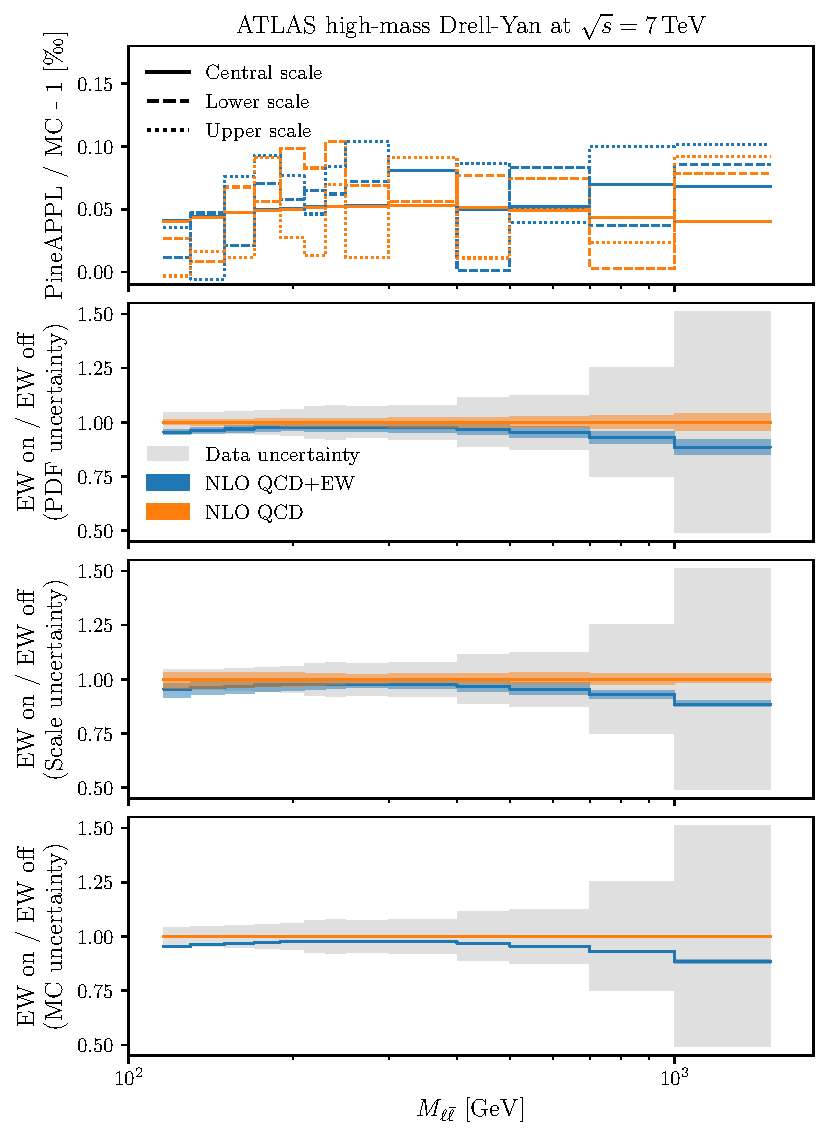
\includegraphics[width=0.5\textwidth]{figures/pineappl_ATLASZHIGHMASS49FB}
    \caption{PineAPPL comparison for ATLAS high-mass Drell--Yan at $\sqrt{s}=7$ TeV.}
    \label{fig:atlaszhighmass49fb}
\end{figure}

\begin{figure}
    \centering
    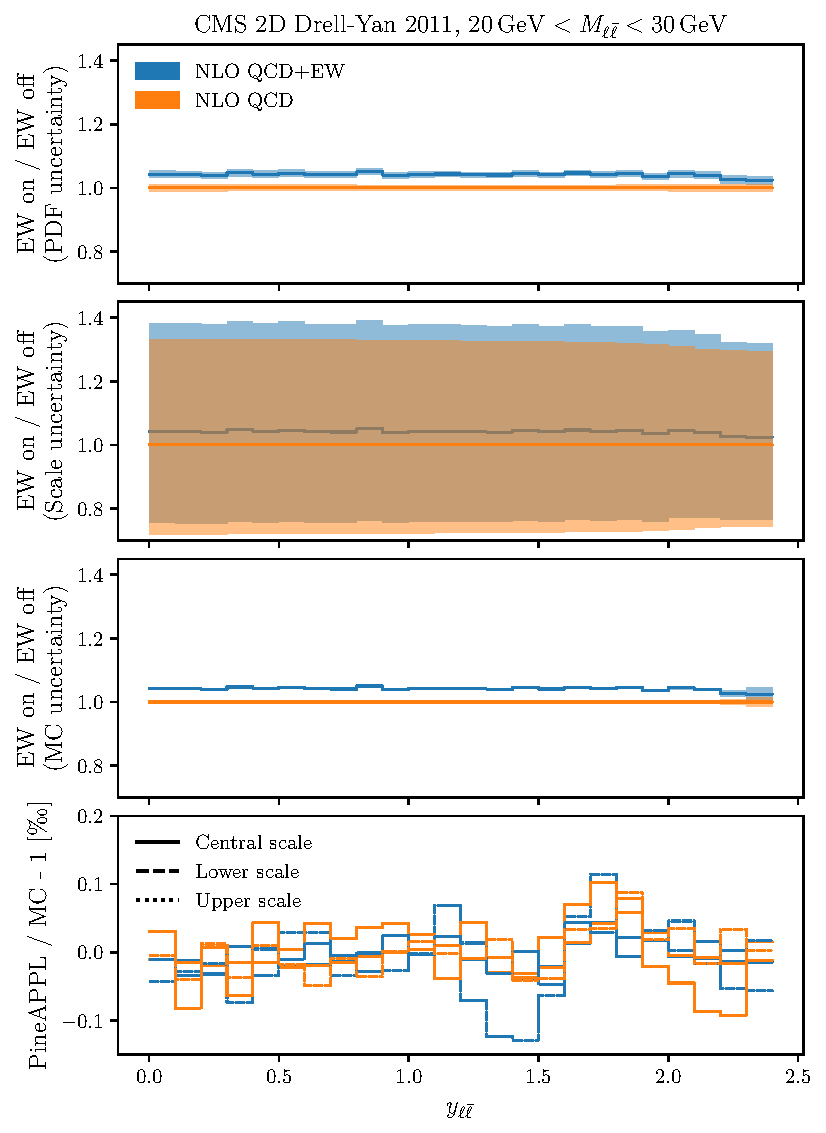
\includegraphics[width=0.5\textwidth]{figures/pineappl_CMSDY2D11_bin1}%
    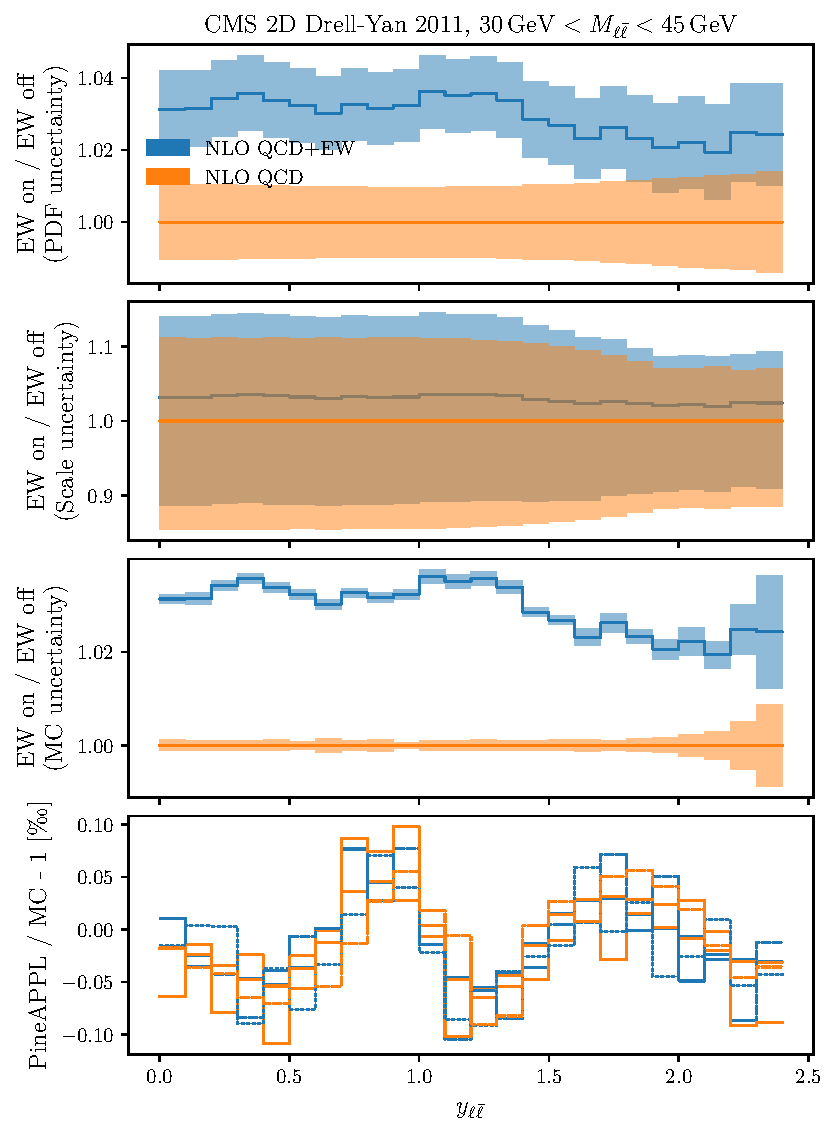
\includegraphics[width=0.5\textwidth]{figures/pineappl_CMSDY2D11_bin2}
    \caption{PineAPPL comparison for CMS 2D Drell--Yan.}
    \label{fig:cmsdy2d11_bins12}
\end{figure}

\begin{figure}
    \centering
    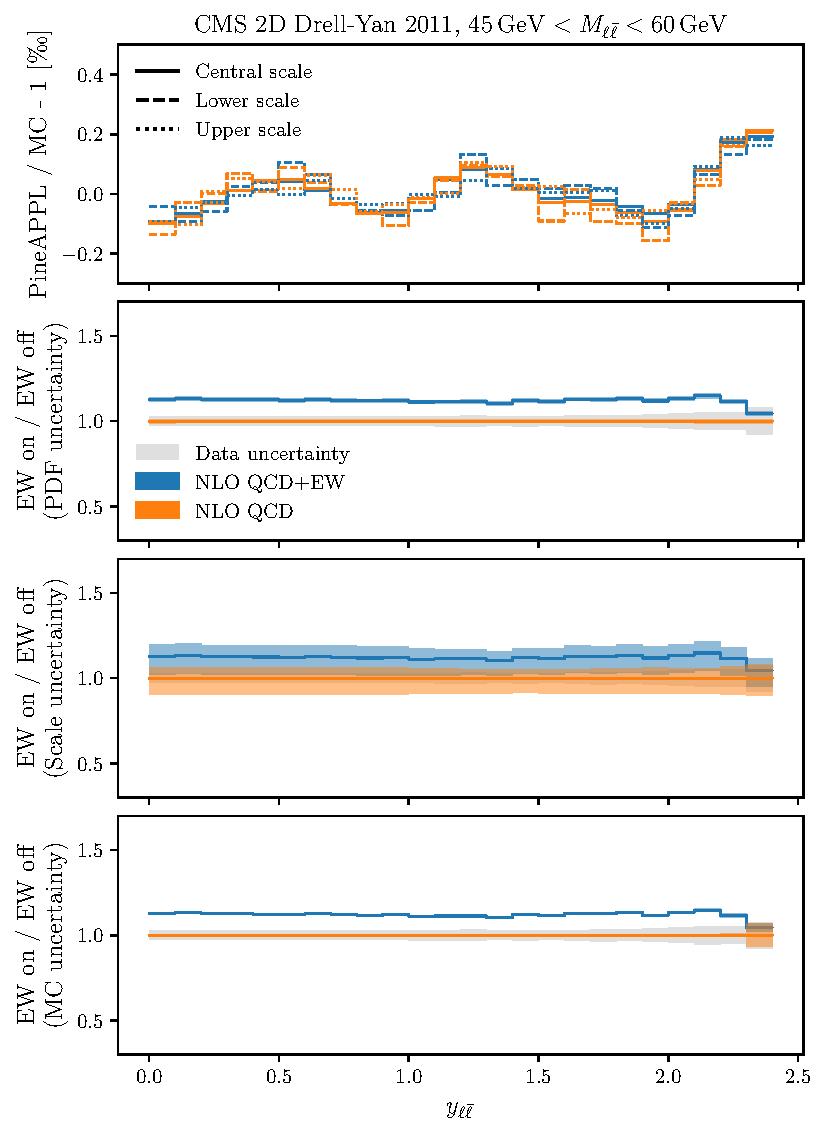
\includegraphics[width=0.5\textwidth]{figures/pineappl_CMSDY2D11_bin3}%
    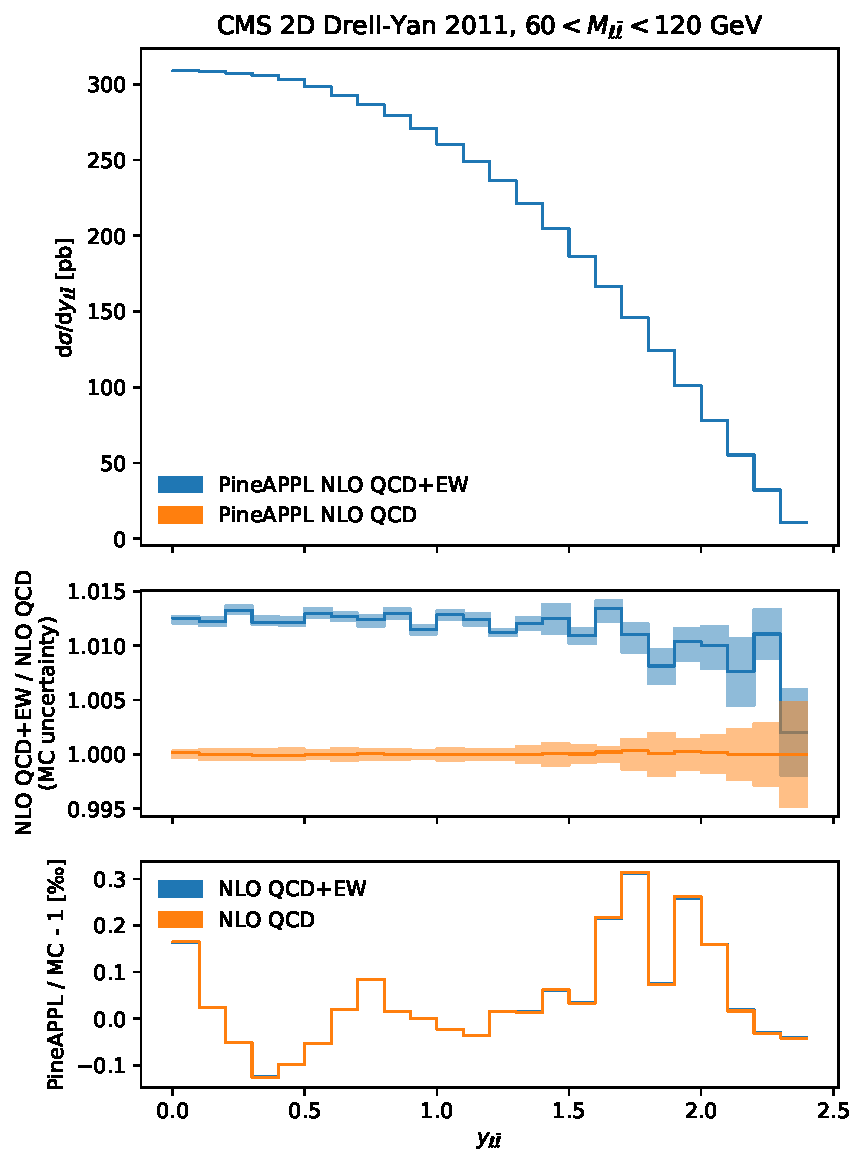
\includegraphics[width=0.5\textwidth]{figures/pineappl_CMSDY2D11_bin4}
    \caption{PineAPPL comparison for CMS 2D Drell--Yan.}
    \label{fig:cmsdy2d11_bins34}
\end{figure}


\begin{figure}
    \centering
    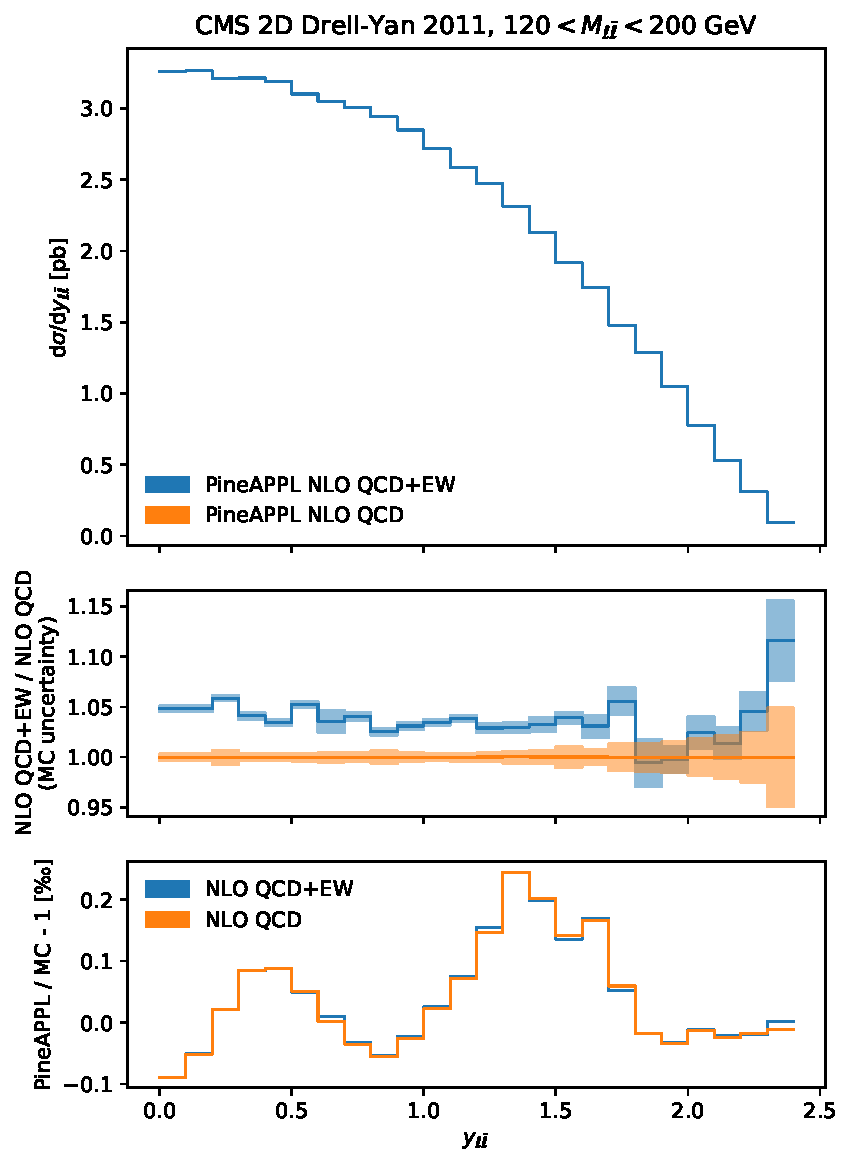
\includegraphics[width=0.5\textwidth]{figures/pineappl_CMSDY2D11_bin5}%
    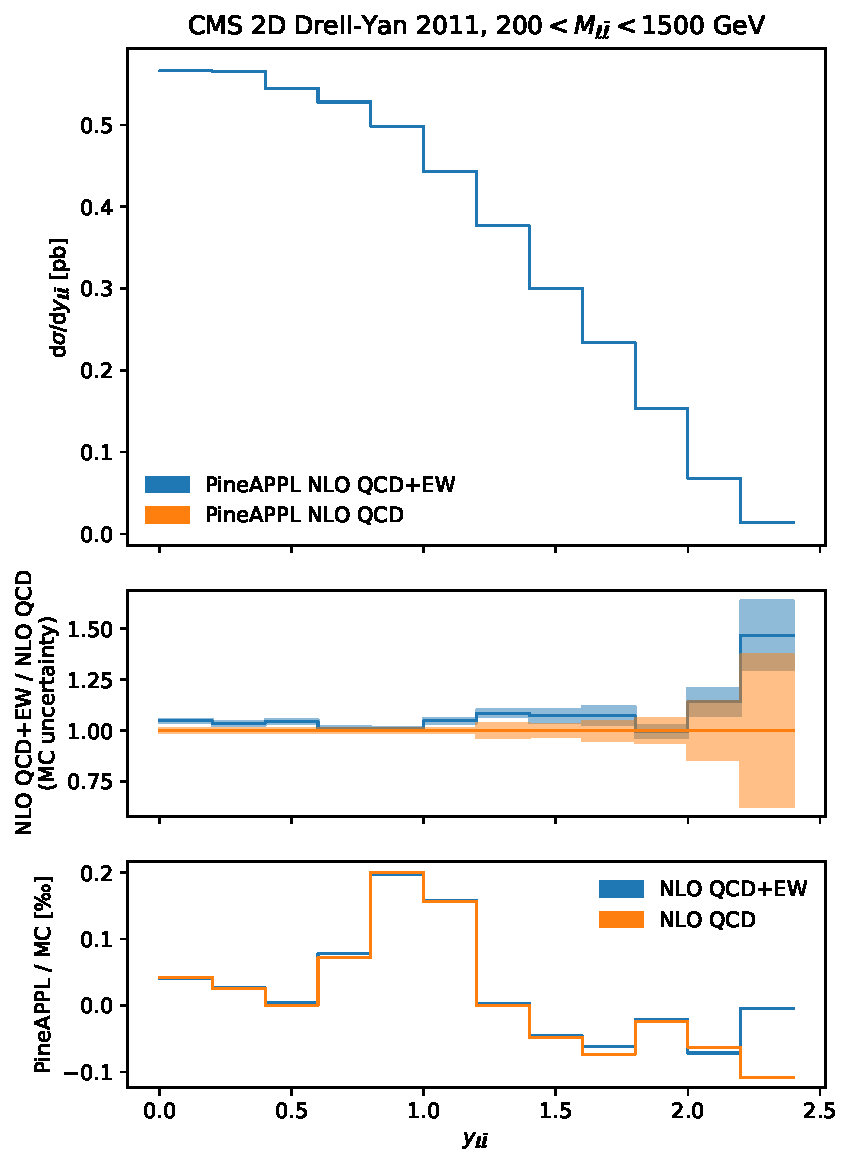
\includegraphics[width=0.5\textwidth]{figures/pineappl_CMSDY2D11_bin6}
    \caption{PineAPPL comparison for CMS 2D Drell--Yan.}
    \label{fig:cmsdy2d11_bins56}
\end{figure}


\begin{figure}
    \centering
    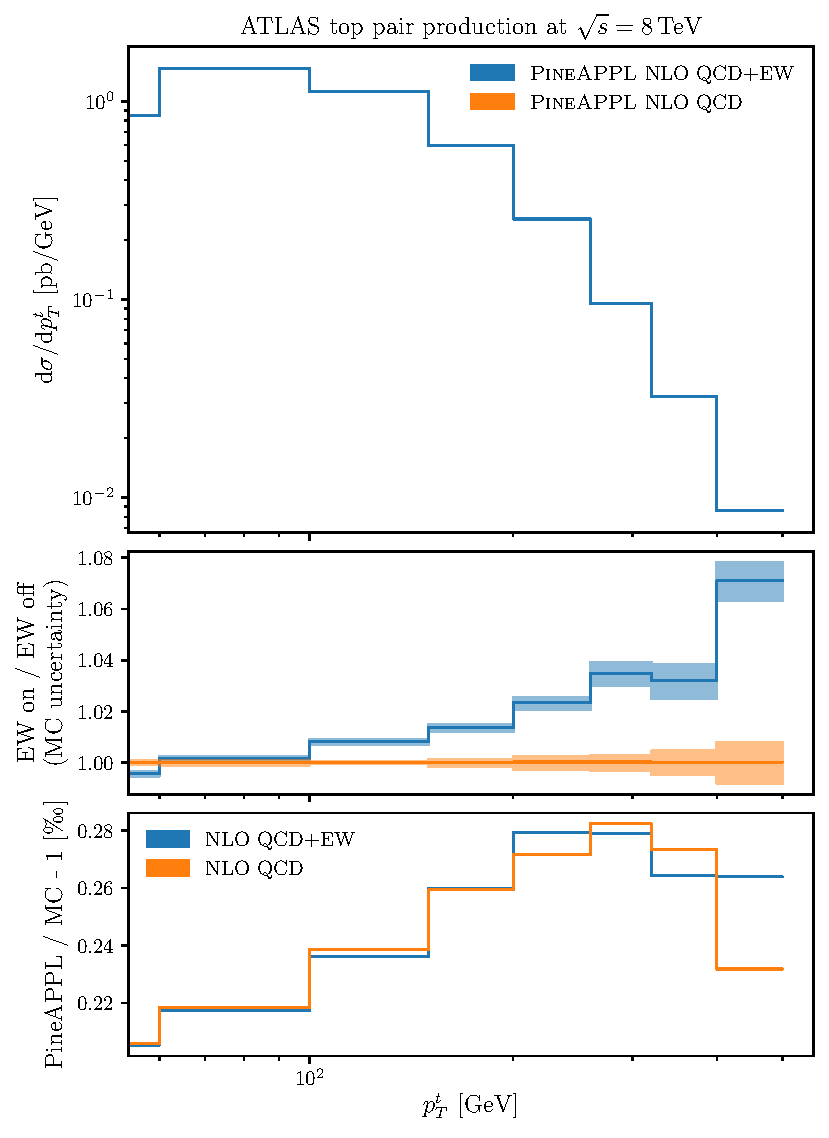
\includegraphics[width=0.5\textwidth]{figures/pineappl_ATLAS_TTB_DIFF_8TEV_LJ_TPT}%
    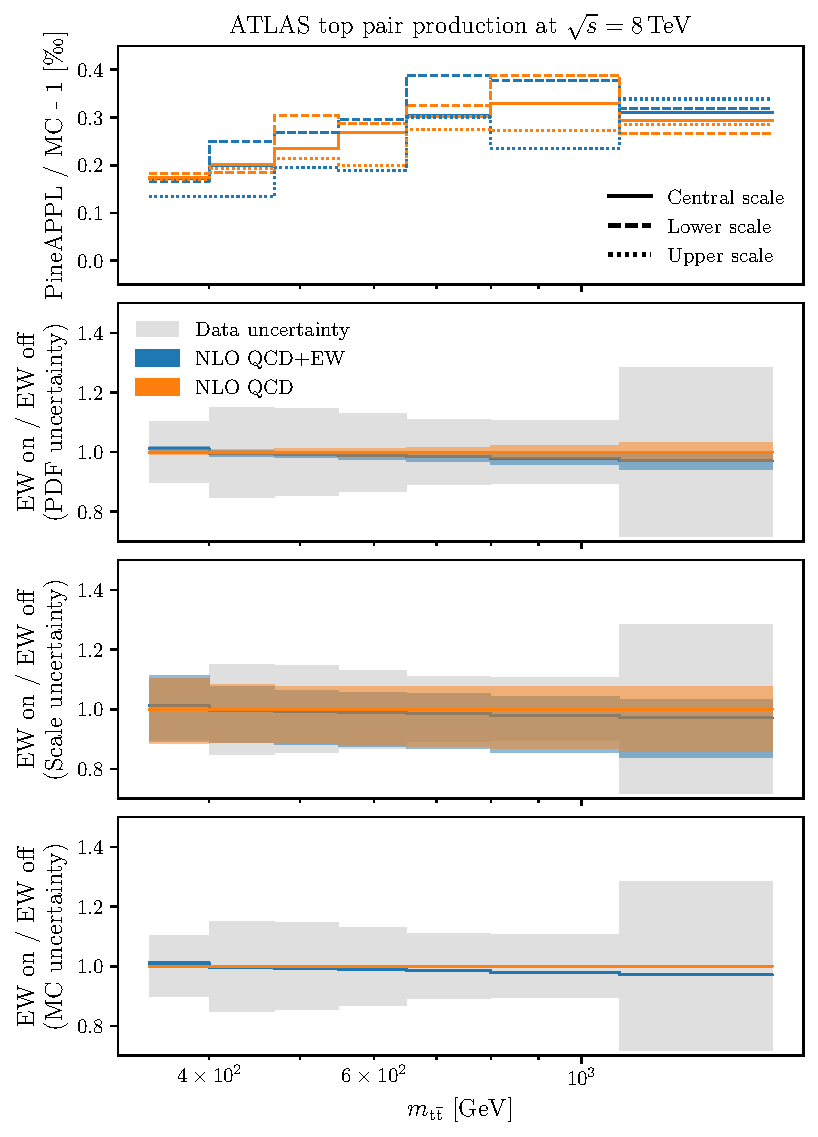
\includegraphics[width=0.5\textwidth]{figures/pineappl_ATLAS_TTB_DIFF_8TEV_LJ_TTM}
    \caption{PineAPPL comparison for ATLAS top pair.}
    \label{fig:cmsdy2d11_bins56}
\end{figure}

\begin{figure}
    \centering
    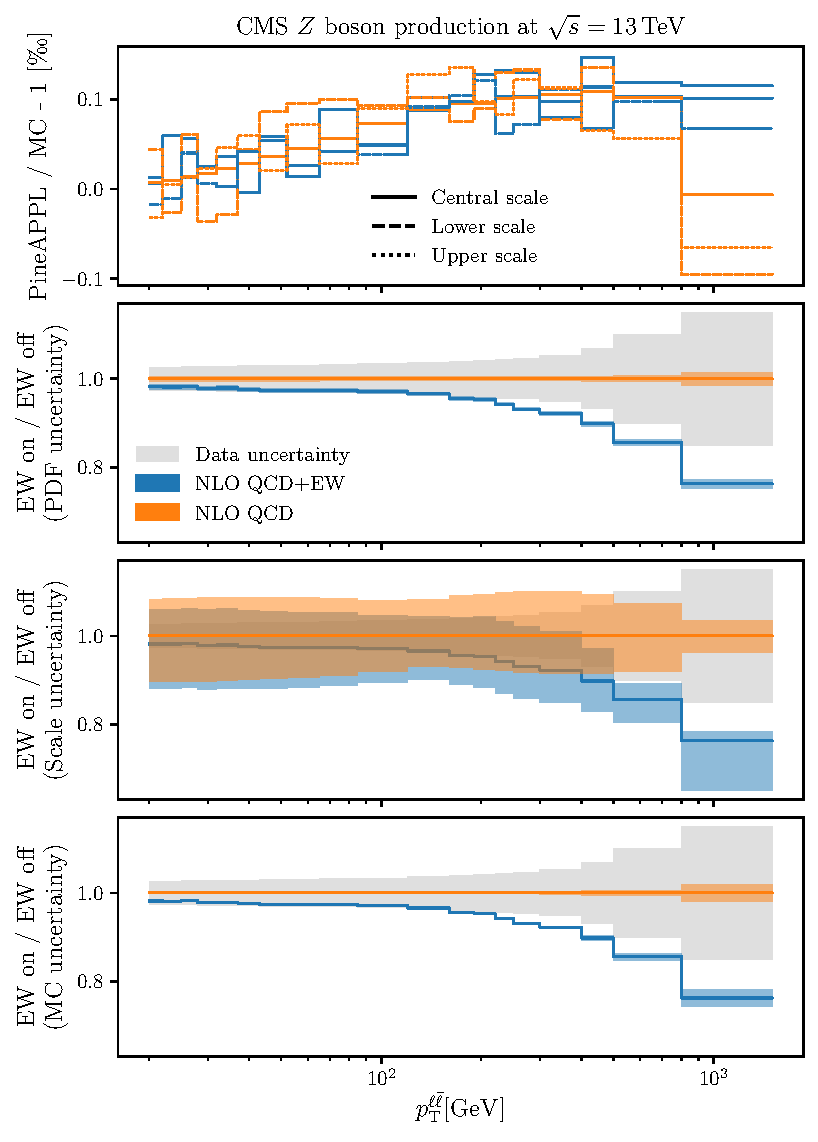
\includegraphics[width=0.5\textwidth]{figures/pineappl_CMS_Z_13_TEV}
    \caption{PineAPPL comparison for CMS $Z$ $p_T$ distribution.}
    \label{fig:cmsdy2d11_bins56}
\end{figure}

\noindent
TODO for each of the following subsections:
\begin{itemize}
\item size of the photon-initiated contributions,
\item largest partonic channel,
\item most important $x$ region,
\item PDF uncertainty,
\end{itemize}




%ERN 7 Apr: there is consensus on the fact that we should present results for the
%following data sets:
%\begin{itemize}
%\item ATLAS high mass DY distributions, 7 TeV~\cite{Aad:2013iua} (CS);
%\item CMS 2D DY distributions, 7 TeV~\cite{Chatrchyan:2013tia} (CS);
%\item ATLAS top pair differential distributions ($m_{t\bar{t}}$ and $p_T^t$),
%8 TeV~\cite{Aad:2015mbv} (ERN);
%\item CMS $Z$ $pT$ distributions, 13 TeV~\cite{Sirunyan:2019bzr} (ERN).
%\end{itemize}
%
%We agree not to display any LHCb measurement, given that they won't add
%further value to our discussion.
%Note added: we might also want to have a look at the ATLAS 2D and 3D DY
%distributions, 8 TeV~\cite{Aad:2016zzw,Aaboud:2017ffb}, if time allows
%us to do so.
%
%CS 25 Jun: We've agreed to show basically two types of plots: 1) technical plots showing the good agreement between the MC compared to the results from the grids, and 2) phenomenological results showing larger EW corrections, for example.
%In the aMCfast paper both is shown in single plot, but since we have more to show, I suggest the following: for the technical plots we show a 2x2 matrix of plots, each showing the difference of the grid result compared to the MC result, in the following fashion:
%\begin{itemize}
%\item NLO QCD with low statistics,
%\item NLO QCD+EW with low statistics,
%\item NLO QCD with high statistics, and finally
%\item NLO QCD+EW with high statistics,
%\end{itemize}
%each showing a few scale variations.
%These plots then clearly show that no matter what corrections you choose, no matter the statistics, and no matter the scale variation, the agreement is always excellent.
%In any case I would like to avoid showing a plot with absolute numbers and low statistics, which looks a bit ridiculous in my opinion (look at figure 1, left side, top plot of the aMCfast paper).
%
%Finally we can show another series of plots, which in my opinion should be very similar to the usual pheno paper plots: absolute numbers with a scale variation band, maybe a few corrections shown in the same plot and then in the bottom relative corrections.
